\documentclass[11pt,a4paper]{article}
\usepackage[a4paper,margin=0.78in]{geometry}
\usepackage[T1]{fontenc}
\usepackage{lmodern}
\usepackage{amsmath,amssymb,booktabs,array}
\usepackage{graphicx}
\usepackage{xcolor,hyperref,enumitem,listings}
\hypersetup{colorlinks=true,linkcolor=blue,urlcolor=blue}
\setlist{nosep,leftmargin=*}
\setlist[description]{style=nextline,leftmargin=0pt}
\emergencystretch=2em
\lstset{basicstyle=\ttfamily\small,breaklines=true,frame=single,backgroundcolor=\color{gray!6}}
\title{Understanding the UVFA Treasure Hunt Project\\\large Task 1, Task 2, and Viva Preparation}
\author{AVD894 Reinforcement Learning Course Project}
\date{November 2026}
\begin{document}
\maketitle
\begin{abstract}
This guide explains the selected paper, the course-project adaptation, its MDPs, exact solver, neural agent, training/evaluation, measured results, limitations, and likely viva questions. The central warning: the project studies a goal-conditioned value-function idea inspired by the paper, but does not reproduce the paper's original experimental environments or results. Be ready to explain both what was implemented and what remains different.
\end{abstract}

\section{The project in one minute}
We study a goal-conditioned grid game. A player starts in a cell, receives a target cell, and must reach it while avoiding walls. In Task 1, we formulate a small version as a finite MDP and solve it with exact value iteration. In Task 2, we build a complete simulator and train one neural action-value model that receives both current state and target. This is related to Universal Value Function Approximators (UVFAs): condition value predictions on goals so one model can serve multiple objectives. The 5,000-episode policy reached 500/500 sampled test episodes on the fixed map and averaged 4.284 moves on successes; a breadth-first-search reference averaged 4.280. These are results for our adaptation, not the original paper benchmark.

\section{The chosen paper}

\subsection{Citation and research question}
Tom Schaul, Daniel Horgan, Karol Gregor, and David Silver, \textquotedblleft Universal Value Function Approximators,\textquotedblright\ Proceedings of the 32nd International Conference on Machine Learning, Proceedings of Machine Learning Research, volume 37, pp. 1312--1320, 2015. Official source: \url{https://proceedings.mlr.press/v37/schaul15.html}.

An ordinary value function $V(s)$ estimates expected future return from state $s$ for one fixed objective. The paper asks how one function can represent values for many goals:
\[
V(s,g;\theta)\approx V_g^\pi(s),\qquad Q(s,a,g;\theta)\approx Q_g^\pi(s,a).
\]
Here $s$ is state, $g$ a goal descriptor, $a$ an action, and $\theta$ shared parameters. The UVFA shares structure across state-goal combinations instead of fitting an unrelated function per goal.

For each goal $g$, the paper defines pseudo-reward $R_g$ and goal-dependent discount $\gamma_g$. The goal value is expected cumulative pseudo-return:
\[
V_g^\pi(s)=\mathbb{E}_\pi\left[
\sum_{t=0}^{\infty}\left(\prod_{k=0}^{t-1}\gamma_g(s_k)\right)
R_g(s_t,a_t,s_{t+1})\ \middle|\ s_0=s\right].
\]
The discount can become zero at goal completion. When a goal is a desired state, the value measures how useful the current state is for reaching that target.

\subsection{What the original paper contributes}
The paper is not simply a DQN paper. It develops:
\begin{enumerate}
\item One goal-conditioned value approximator, $V(s,g)$ or $Q(s,a,g)$.
\item Two-stream representations: state maps to $\phi(s)$, goal to $\psi(g)$, and a function $h$ combines them. It also studies concatenating state and goal.
\item Supervised low-rank factorization: known values form a state-by-goal matrix; factorization produces target embeddings; networks learn state/goal-to-embedding mappings. The paper reports faster learning than naive regression in its experiments.
\item Reinforcement-learning approaches: a Horde of goal-specific value learners can provide targets for a UVFA; another method directly bootstraps a UVFA with a Q-learning variant.
\item Generalization evaluations in gridworld/LavaWorld and Ms. Pac-Man. One four-room experiment trained on goals in three rooms and tested in the fourth, reporting policy quality $24\%\pm8\%$. The Ms. Pac-Man study used pellet coordinates as goals; it trained from 29 goal-specific learners and examined five unseen pellet goals.
\end{enumerate}
The paper's contribution is transfer across goal-conditioned value functions. Its environments, training procedures, and evaluation metrics are part of the experiment and must match before claiming reproduction.

\section{Original paper versus our implementation}
\begin{center}
\small
\begin{tabular}{p{0.22\linewidth}p{0.35\linewidth}p{0.35\linewidth}}
\toprule
Aspect & Schaul et al. (2015) & Course project\\
\midrule
Function & $V(s,g)$ and/or $Q(s,a,g)$ shares parameters & Neural $Q(s,g,\cdot)$ returns four movement values\\
Architecture & Concatenation, two-stream embeddings, low-rank factorization & Separate MLP state/goal encoders, concatenate embeddings, MLP Q-head\\
Learning & Supervised factorization; Horde targets; or direct UVFA bootstrap & DQN-style Q-learning, replay, target network, Huber loss\\
Environment & Paper gridworld/LavaWorld and Atari Ms. Pac-Man & Custom symbolic 8-by-8 treasure maze\\
Generalization & Some experiments hold out goals & Fresh random episode seeds on same map; goal cells are not held out\\
Metrics & Paper-specific MSE and policy quality & Success, path length, return in custom maze\\
\bottomrule
\end{tabular}
\end{center}
This is a \textbf{UVFA-inspired adaptation}, not an exact reproduction. Task 1 value iteration is the course's exact-MDP exercise, not a paper result. Replay, target-network updates, Huber loss, and reward shaping are implementation choices.

\section{Task 1: optimization problem and exact MDP}

For a fixed maze and target, find a policy $\pi$ that reaches the target while avoiding collisions and unnecessary movement. With negative movement/collision costs and positive terminal reward:
\[
\pi^*=\arg\max_\pi J(\pi),\qquad
J(\pi)=\mathbb{E}_\pi\left[\sum_{t=0}^{T-1}\gamma^t r_t\right].
\]
The Task 1 map has 22 free cells. A nonterminal state is player position $p$ and target $g$, $p\ne g$:
\[
\mathcal{S}=\{(p,g):p,g\in\mathcal{C},p\ne g\},\quad
|\mathcal{S}|=22\cdot21=462.
\]
Actions are up/down/left/right. A legal move changes position to an adjacent free cell; an attempt into a wall leaves position unchanged. Reward:
\[
r(s,a,s')=\begin{cases}
+10 & \text{reaches goal},\\
-0.1 & \text{legal nonterminal move},\\
-1 & \text{wall collision}.
\end{cases}
\]
The episode terminates at the goal and $\gamma=0.95$.

Value iteration applies the Bellman optimality update:
\[
V_{k+1}(s)=\max_a[r(s,a,T(s,a))+\gamma V_k(T(s,a))].
\]
Updates are synchronous. It stops when $\Delta_k=\max_s|V_{k+1}(s)-V_k(s)|<10^{-10}$ or the iteration cap is reached. The greedy policy selects the maximizing action. Measured Task 1 result: 462 pairs, four actions, convergence in 10 iterations, final delta 0.0, and a 9-move example path from $(1,1)$ to $(5,6)$. See \texttt{docs/report1\_task1.pdf} and \texttt{artifacts/task1/}.

\section{Task 2: simulator MDP and reward}

The Task 2 map is 8-by-8 with 33 free cells, giving $33\cdot32=1,056$ nonterminal ordered position-goal pairs. At episode start, two distinct free cells are sampled.

The conceptual state is $s_t=(p_t,g)$. If the 50-step horizon is part of the task, a fully Markov finite-horizon state should also include remaining time: $(p_t,g,50-t)$. Four actions move up/down/left/right. Goal achievement terminates; hitting the 50-step cap truncates.

\textbf{Network input size is not state count.} The state vector has 128 values: 64 one-hot entries for agent location and 64 entries for the obstacle map. The goal vector is a separate 64-dimensional one-hot encoding. The map is fixed, so obstacle bits are constant during training. This encoding can carry map information, but map generalization was not evaluated. Remaining time is not an input, so the learned policy is stationary near the truncation boundary.

Base rewards are $+10$ for goal, $-0.1$ for legal motion, and $-1$ for a wall attempt. A legal nonterminal move adds Manhattan-distance shaping:
\[
r'_t=-0.1+0.15(d_t-d_{t+1}).
\]
The goal transition receives $+10$ directly; wall attempts receive $-1$ without shaping. This is a disclosed adaptation. It uses raw Manhattan-distance change, not a formally specified potential-based shaping term, so policy invariance is not established. Obstacles can make Manhattan and true shortest-path distances differ. Task 1 remains unshaped.

\section{Task 2 agent and learning}

\subsection{Network and policy}
Let $x(s)$ be the 128-dimensional state encoding and $z(g)$ the 64-dimensional target encoding. Separate encoders produce $e_s=f_s(x(s))$ and $e_g=f_g(z(g))$. An MLP maps their concatenation to four Q-values:
\[
\mathbf{Q}_\theta(s,g)=h_\theta([e_s,e_g])\in\mathbb{R}^4,\qquad
Q_\theta(s,g,a)=\mathbf{Q}_\theta(s,g)_a.
\]
Each encoder has a 128-unit layer and 64-dimensional embedding. The head maps the concatenated 128 embedding values through 128 hidden units to four actions. At test time choose $\arg\max_a Q(s,g,a)$. During training epsilon-greedy chooses a random action with probability $\epsilon$, otherwise greedy.

\subsection{TD target, loss, stabilizers}
Replay stores $(s_t,g,a_t,r_t,s_{t+1},g,d_t)$. The goal stays fixed in an episode. A target network provides:
\[
y_t=r_t+\gamma(1-d_t)\max_{a'}Q_{\theta^-}(s_{t+1},g,a').
\]
$d_t=1$ for terminal or truncated transitions. TD error is $\delta_t=Q_\theta(s_t,g,a_t)-y_t$. Smooth-L1/Huber loss is
\[
L(\theta)=\begin{cases}
\frac12\delta_t^2&|\delta_t|\le1,\\
|\delta_t|-\frac12&|\delta_t|>1.
\end{cases}
\]
Replay reduces adjacent-transition correlation and reuses experience. The target network is hard-copied every 100 environment steps. Adam updates the online network; gradient norm is clipped at 5. These are DQN-style adaptations, not the paper's exact algorithm.

\subsection{Training configuration}
\begin{center}
\small
\begin{tabular}{ll}
\toprule
Parameter & Value\\
\midrule
Map & Fixed 8-by-8; 33 free cells\\
Episodes & 1,000 baseline; 5,000 extended\\
Seed & 2026; episode $i$ uses $2026+i$\\
Data & None downloaded; episodes generated online\\
Maximum episode length & 50\\
Discount & 0.95\\
Adam learning rate & 0.001\\
Replay capacity / batch & 20,000 / 64\\
Warm-up & 200 transitions\\
Target update / train frequency & 100 steps / every step\\
Epsilon & 1.0 to 0.05 over 5,000 environment steps\\
Shaping scale & 0.15 times Manhattan-distance change\\
Hardware & NVIDIA RTX 3050 Laptop GPU\\
Software & Python 3.12.4; PyTorch 2.5.1+cu121; NumPy 2.4.6\\
\bottomrule
\end{tabular}
\end{center}
In RL, count episodes, environment steps, and gradient updates rather than epochs over labelled data. The 5,000 run generated 28,770 transitions and 28,571 optimizer updates. Test seeds were 100000--100499; training episode seeds start at 2026.

\section{Evaluation and meaning of results}
Both checkpoints were evaluated on the same 500 episode seeds. Each episode samples a start and target from the same map. The BFS baseline searches the known maze for a shortest path. It is not an RL agent and has explicit map access.

\begin{center}
\small
\begin{tabular}{p{0.30\linewidth}rrr}
\toprule
Metric & 1,000 episodes & 5,000 episodes & BFS\\
\midrule
Success & 493/500 = 98.6\% & 500/500 = 100\% observed & 500/500\\
Success Wilson 95\% interval & 97.14--99.32\% & 99.24--100.00\% & --\\
Mean moves on successful episodes & 4.546 & 4.284 & 4.280\\
Mean return & 9.9012 & 10.1378 & 10.1382\\
\bottomrule
\end{tabular}
\end{center}
Successful-path bootstrap 95\% intervals (20,000 resamples, seed 2026): 4.349--4.744 moves for 1,000 episodes; 4.104--4.466 for 5,000. They overlap, so do not claim statistical separation of the conditional means. 100\% observed success does not prove perfect future performance; the Wilson lower bound is 99.24\%.

\begin{figure}[ht]
\centering
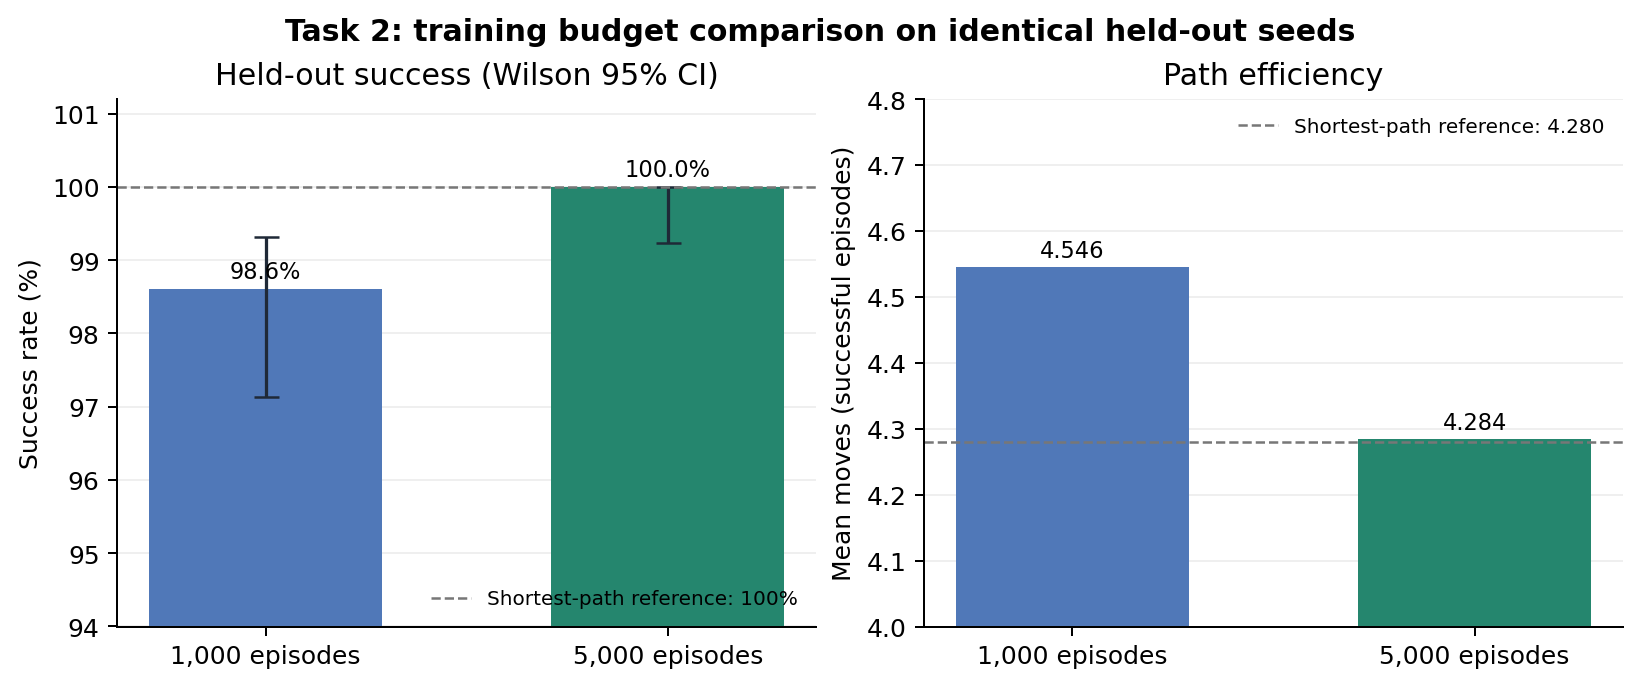
\includegraphics[width=0.92\linewidth]{task2_training_comparison.png}
\caption{Matched-seed training-budget comparison. Error bars in the success panel are Wilson 95\% intervals; the other panel compares conditional successful path length.}
\end{figure}
The longer run improved the measured result on this fixed map and sample. There is one training seed. This does not establish robustness across training seeds, new-map generalization, or reproduction of the paper's MSE/policy-quality results.

\section{Reproduction status: the honest answer}
The course expects paper understanding and reproduction where possible. This project implements the central goal-conditioned value idea in a simulator, but it does \textbf{not} reproduce Schaul et al.'s original experimental results.

\begin{itemize}
\item \textbf{Implemented:} a single model conditions action values on state and goal; separate encoders; custom simulator; exact Task 1 reference; training/evaluation; fresh episode seeds; demo.
\item \textbf{Changed:} custom maze instead of paper environments; DQN-style replay/target network/Huber instead of the paper's specific supervised factorization, Horde, or direct-bootstrap experiment; custom rewards and shaping; different metrics.
\item \textbf{Not tested:} a disjoint set of goal cells absent from training, independent training seeds, new maps, or original paper benchmarks.
\end{itemize}
Fresh random test seeds create new \emph{episodes}, but goals come from the same set as training and position-goal pairs may reoccur. Do not call this strict held-out-goal generalization. The next useful experiment is to reserve specific goal cells from all training episodes, evaluate on those goals, and repeat over several training seeds. A closer paper reproduction requires an original environment and its corresponding algorithm/metric.

\section{Code map and demo}
\begin{itemize}
\item \texttt{configs/task1\_small.json}, \texttt{configs/task2\_default.json}: map and settings.
\item \texttt{src/goal\_treasure/env.py}: reset, step, encodings, rewards, termination.
\item \texttt{src/goal\_treasure/exact.py}: value iteration and Task 1 rollout.
\item \texttt{src/goal\_treasure/uvfa.py}: network, replay, action selection, TD update, checkpoints.
\item \texttt{scripts/run\_task1.py}: exact Task 1; \texttt{scripts/train\_task2.py}: training.
\item \texttt{scripts/evaluate\_task2.py}: test and BFS comparison; \texttt{scripts/demo.py}: Tkinter interface.
\item \texttt{notebooks/AVD894\_Task1\_Task2.ipynb}: notebook workflow and results.
\end{itemize}
In the window, \textbf{Next RL step} advances one greedy action; \textbf{Auto-play} animates; \textbf{Pause} stops; \textbf{New random episode} samples another start/goal. Blue is agent, green target, grey walls, light blue visited path. The panel shows action, reward, return, and move count.

\section{Viva questions and model answers}
\begin{description}
\item[What is the paper's question?] Can one value approximator represent and generalize values across states and goals?
\item[Why one UVFA rather than one model per target?] Shared parameters can reuse structure between related states and goals.
\item[What does universal mean?] One parameterized approximator for a specified goal set; it is not guaranteed to solve all goals or environments.
\item[How does a goal differ from a task?] A goal changes reward while dynamics stay fixed; a task may change MDP dynamics.
\item[How many Task 1 decision states?] 22 free positions times 21 other goals = 462 ordered state-goal pairs.
\item[Why value iteration?] The finite model is small and known, so Bellman updates give an exact transparent reference.
\item[What does the Task 2 network output?] Four action values conditioned on agent/map and target encodings.
\item[What is the TD target?] Observed reward plus discounted target-network next value, except on terminal/truncated transitions.
\item[Why replay and target networks?] Replay reduces adjacent-sample correlation and reuses data; the target network slows bootstrap changes.
\item[Why Huber loss?] Quadratic for small TD errors and linear for large ones, reducing sensitivity to outliers.
\item[What is BFS?] A shortest-path planner with known-map access, not another RL method.
\item[Was a dataset downloaded?] No, episodes are generated online by the simulator.
\item[Does 100\% on 500 episodes prove perfect generalization?] No; one map and one training seed, and the Wilson lower bound is 99.24\%.
\item[Did we reproduce the original paper?] No. We adapted its goal-conditioned value idea but changed environment, learning details, rewards, and metrics.
\item[What is the strongest next experiment?] Hold out goal locations during training and use multiple independent training seeds.
\end{description}

\section{Sources}
\begin{enumerate}
\item Schaul, T., Horgan, D., Gregor, K., and Silver, D. (2015). Universal Value Function Approximators. ICML, PMLR 37, 1312--1320. \url{https://proceedings.mlr.press/v37/schaul15.html}
\item AVD894 Course Project and Term Paper instructions supplied for this project, especially Intermediate Tasks 1 and 2.
\item Project measurements in \texttt{docs/RESULTS.md} and local \texttt{artifacts/} outputs.
\end{enumerate}
\end{document}
